% Created 2025-11-01 Sat 16:56
% Intended LaTeX compiler: pdflatex
\documentclass[11pt,twocolumn]{article}
\usepackage[utf8]{inputenc}
\usepackage[T1]{fontenc}
\usepackage{amsmath}
\usepackage{amssymb}
\usepackage{capt-of}
\usepackage{hyperref}
\usepackage{geometry}
\geometry{margin = 1cm}

%% ox-latex features:
%   !announce-start, !guess-pollyglossia, !guess-babel, !guess-inputenc,
%   maths, image, !announce-end.

\usepackage{amsmath}
\usepackage{amssymb}

\usepackage{graphicx}

%% end ox-latex features


% end precompiled preamble
\ifcsname endofdump\endcsname\endofdump\fi

\author{Niraj Kumar Singh , Roll No : AM25M807}
\title{STEADY 2D Convection - Diffusion}
\hypersetup{
 pdfauthor={Niraj Kumar Singh , Roll No : AM25M807},
 pdftitle={STEADY 2D Convection - Diffusion},
 pdfkeywords={},
 pdfsubject={},
 pdfcreator={},
 pdflang={English}}
\begin{document}

\maketitle

\section{STEADY  2D  - Convection  - Diffusion}
\label{sec:orgb6eb954}
The two-dimensional transport equation for temperature reads
\[\frac{\delta}{\delta x}(\rho U T) + \frac{\delta}{\delta y} (\rho V T)  = \frac{\delta}{\delta x} (\gamma \frac{\delta T}{\delta x}  ) + \frac{\delta}{\delta y} (\gamma \frac{\delta T}{\delta Y}) + S\]

where
\[ \gamma = \frac{\rho}{C_p} \]
\section{Simulation result with error tolerance of  error < 0.0001}
\label{sec:orge1eb83b}
\begin{center}
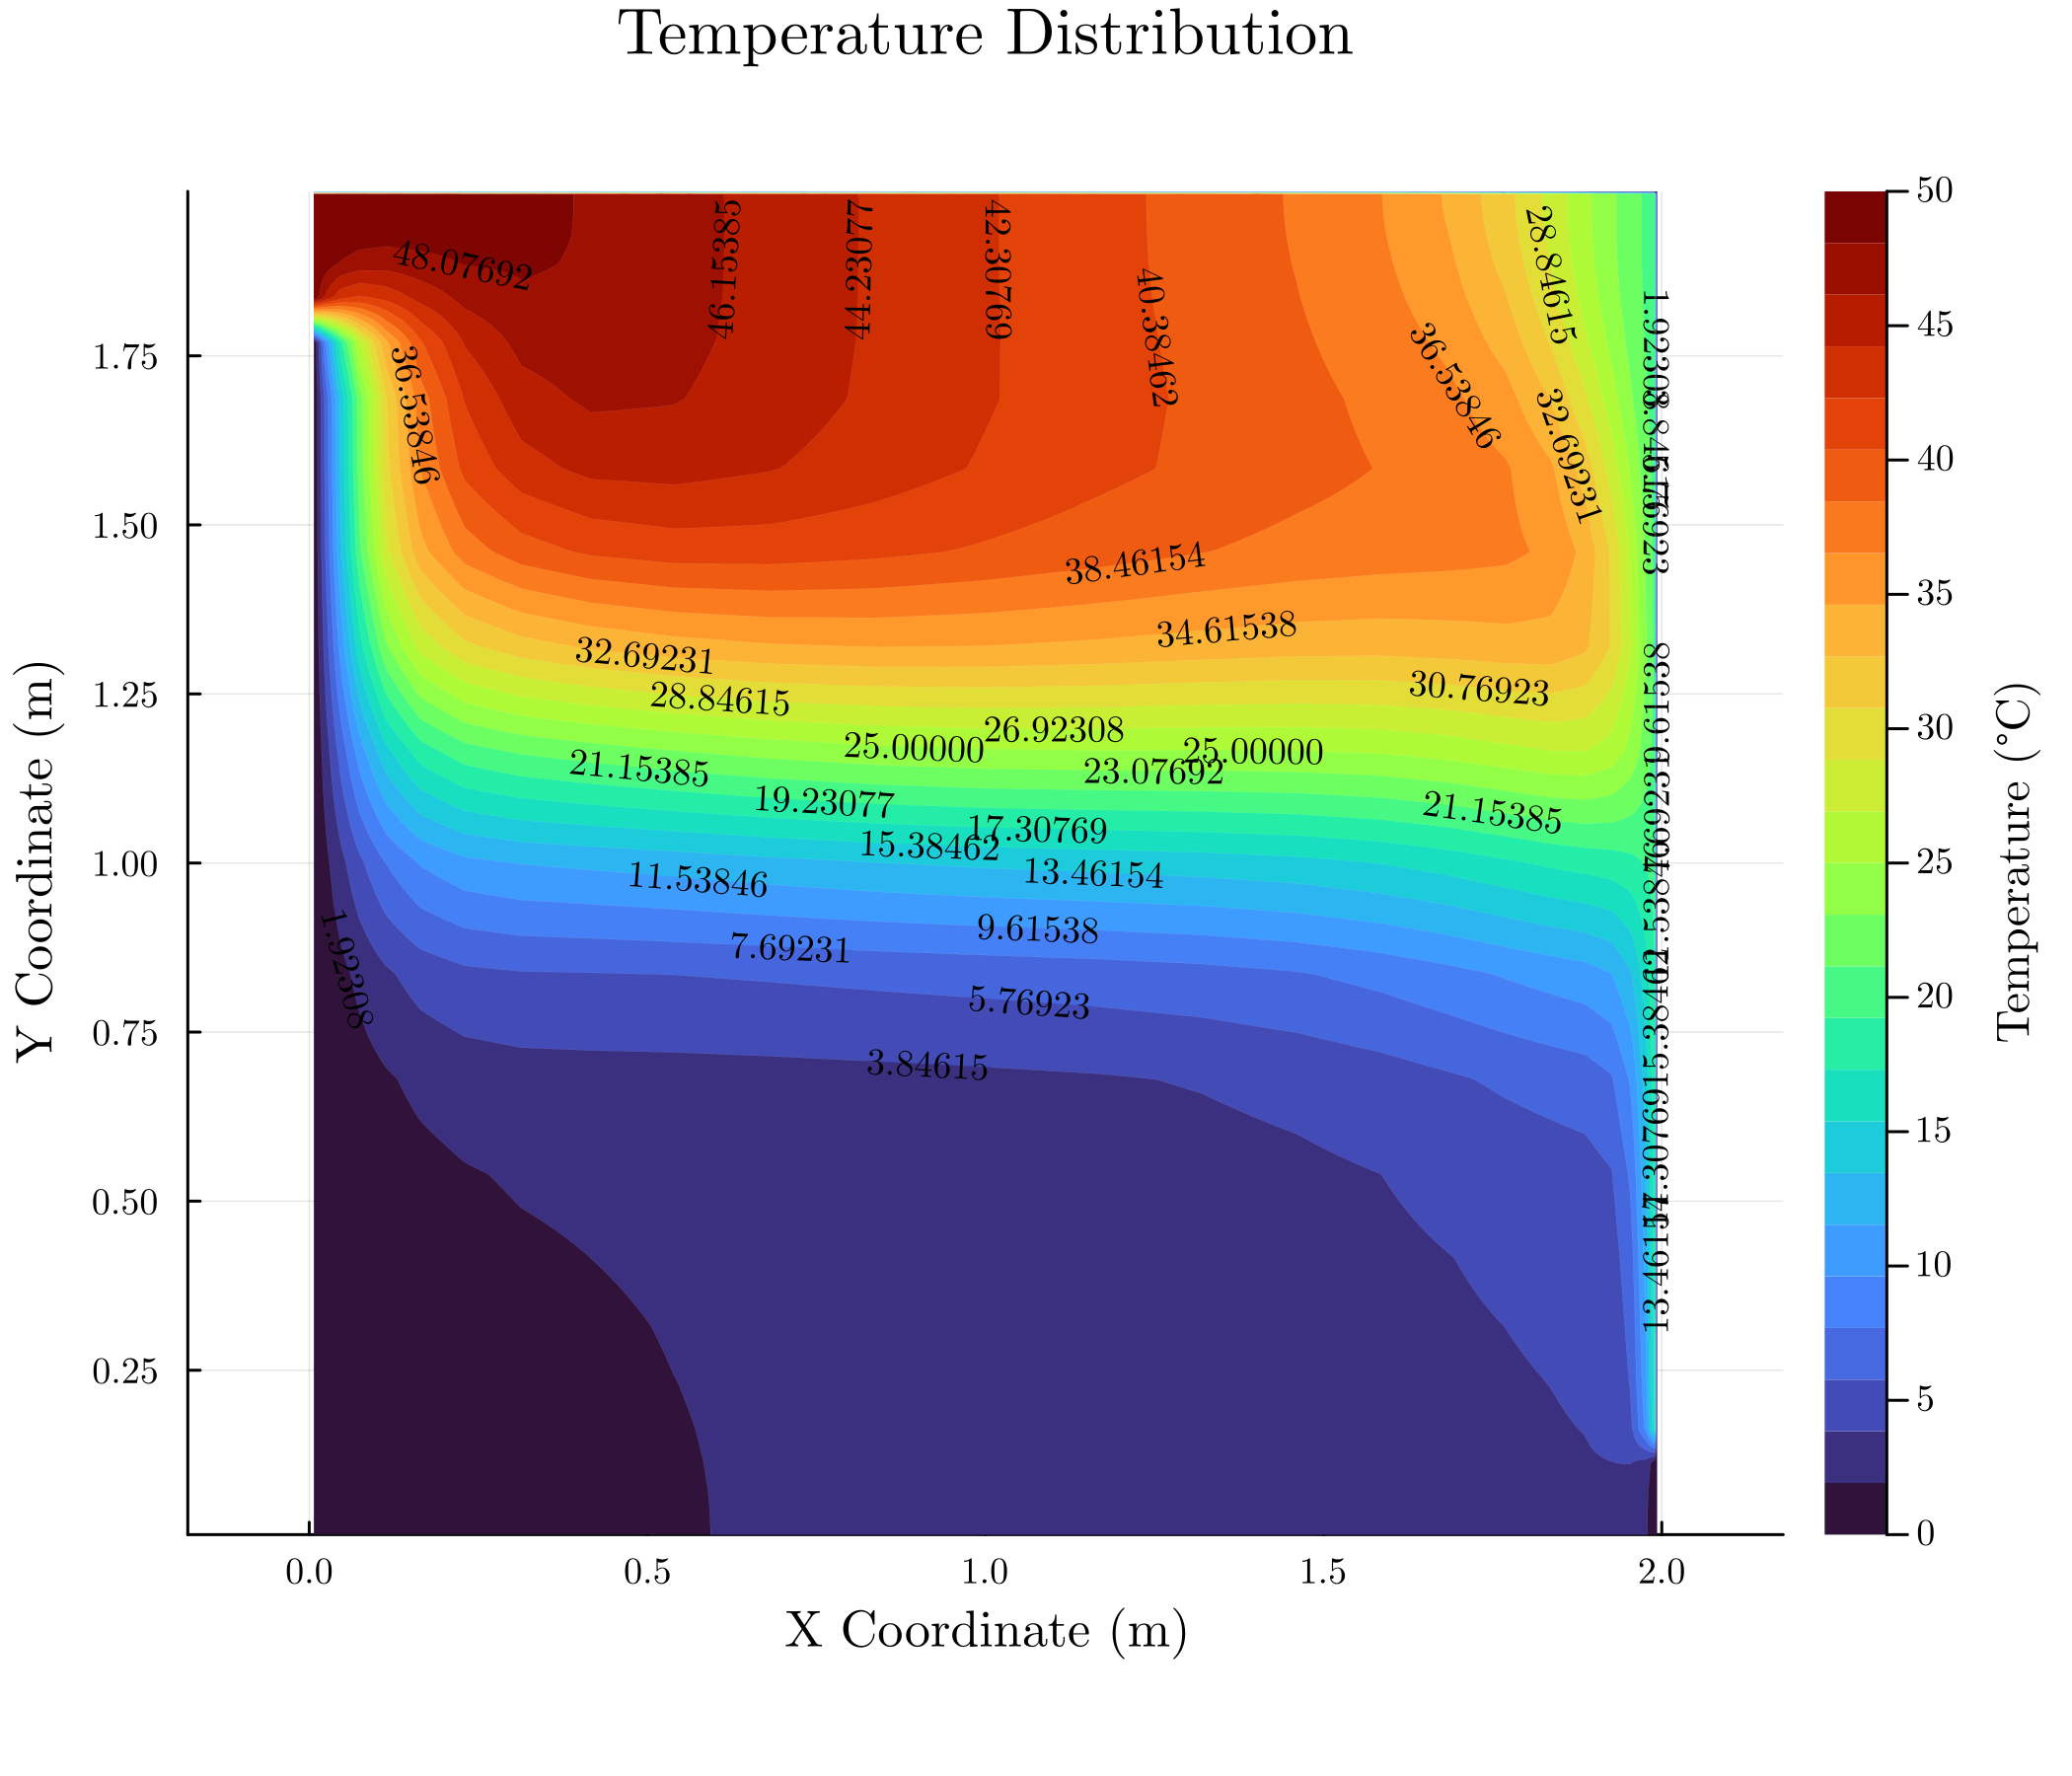
\includegraphics[width=.9\linewidth]{./result.png}
\end{center}
\section{Sensitivity to Boundary Condition}
\label{sec:org653d2bd}
At East Boundary , except at outlet Temperature is fixed  at 50 degree
The Dirichlet conditon [T = 50 degree C]is applied at East Boundary except at the outlets which was previously set to [T = 20 degree C] 

\begin{center}
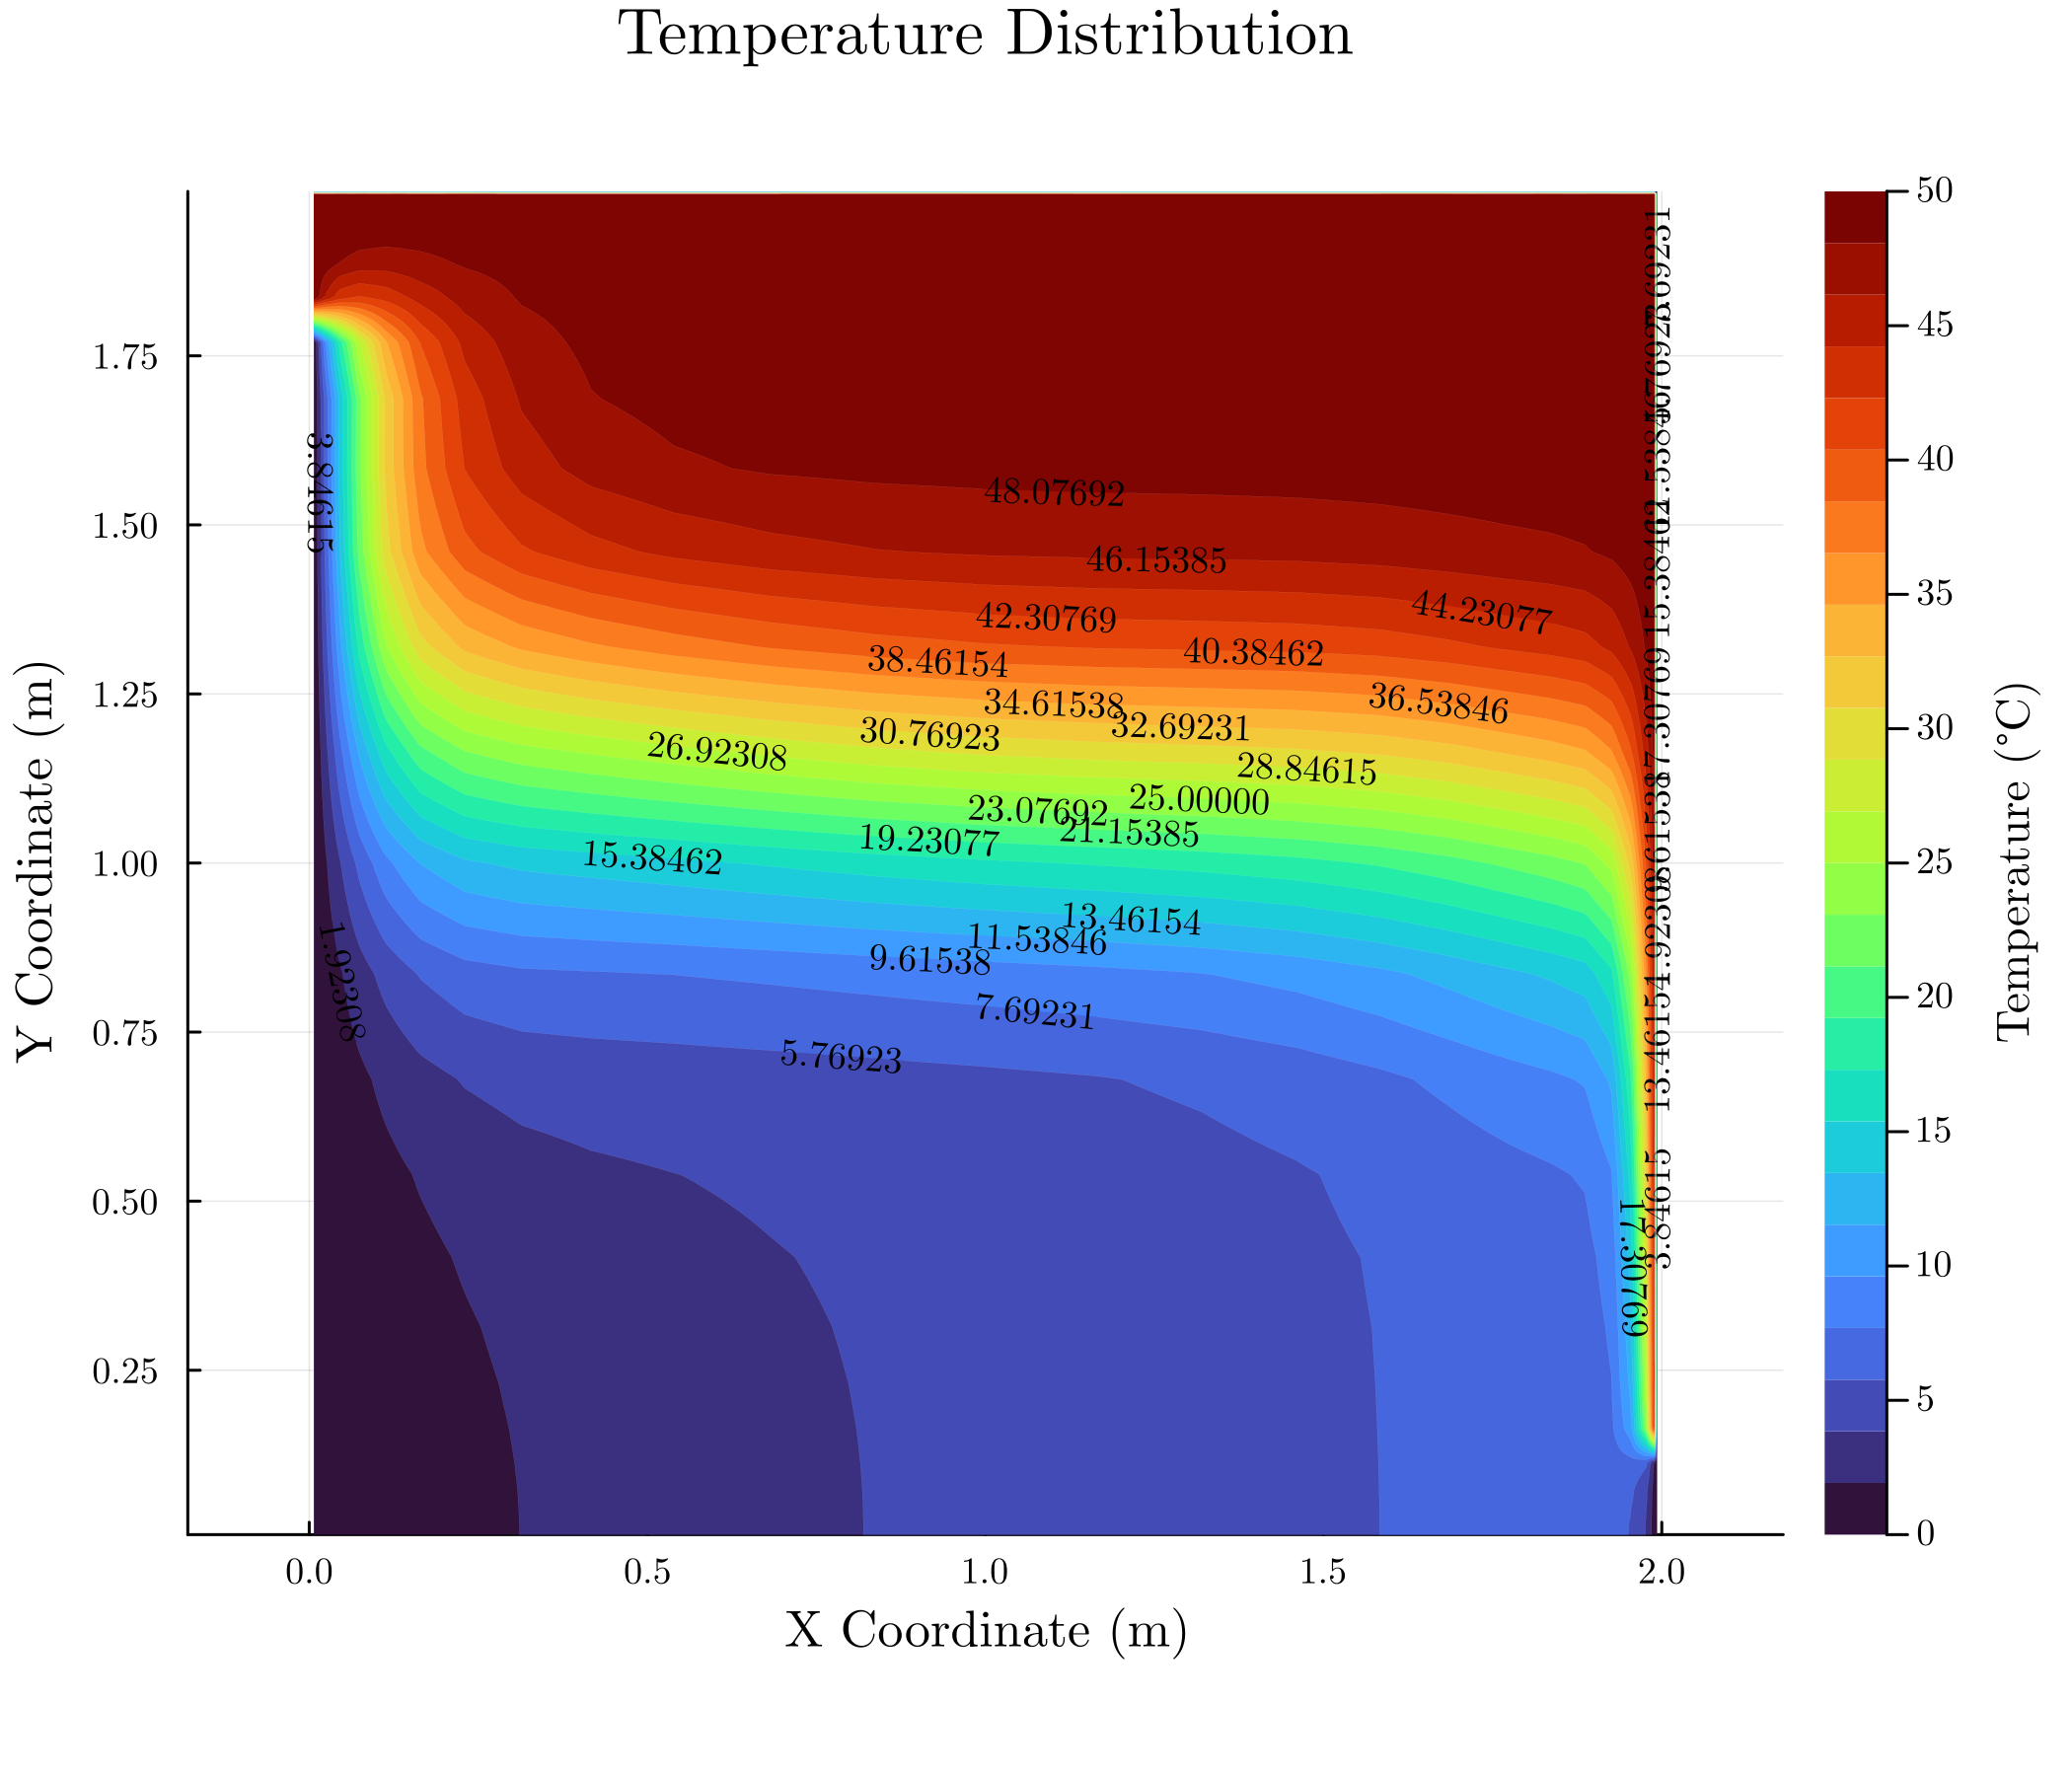
\includegraphics[width=.9\linewidth]{./result1.png}
\end{center}
\section{Sensitivity to Convergence}
\label{sec:orga8ab013}

\subsection{TDMA Convergence Test}
\label{sec:org33d2d2c}
\begin{center}
\begin{tabular}{lrrrrrrrr}
tolerance Value & 10.0 & 1.0 & 0.1 & 0.001 & 0.0001 & 1.0e-5 & 1.0e-6 & 1.0e-7\\
counter & nil & nil & 10.0 & 126.0 & 256.0 & 297.0 & 298.0 & 297.0\\
\end{tabular}
\end{center}
\begin{center}
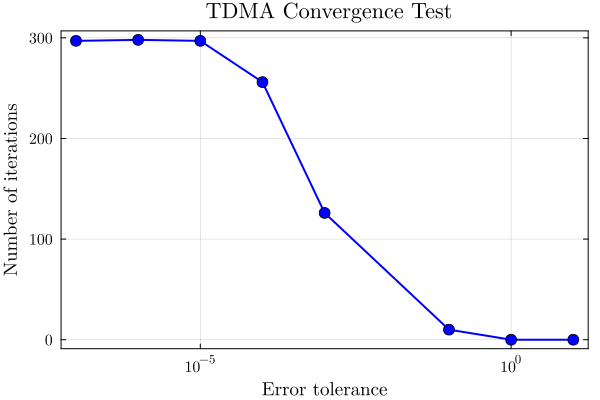
\includegraphics[width=.9\linewidth]{./conv.png}
\end{center}
\subsection{Gauss-Siedel Convergence Test}
\label{sec:orge8d958a}

\begin{center}
\begin{tabular}{lrrrrrrrr}
tolerance Value & 10.0 & 1.0 & 0.1 & 0.001 & 0.0001 & 1.0e-5 & 1.0e-6 & 1.0e-7\\
Counter & nil & nil & 4 & 133 & 1277 & 12865 & 17840 & 17840\\
\end{tabular}
\end{center}

\begin{center}
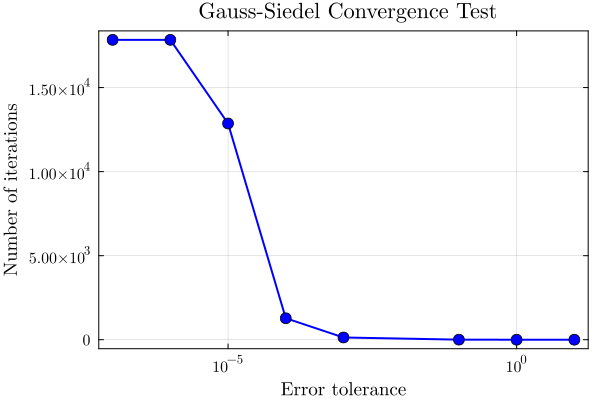
\includegraphics[width=.9\linewidth]{./conv1.png}
\end{center}

Comments : TDMA converges much faster for error tolerance 1e-7 297 iteration are performed for solution to converge , but for Gauss Siedel 17840 iteration are performed for same error tolerance   
\end{document}
